% -*- coding: utf-8; -*-

\chapter{Resultados}
\label{ch:result}

	Este capítulo apresenta os resultados desta dissertação para volumes de malhas regulares conhecidos na literatura e simulações de reservatório de petróleo, respectivamente nas Seções~\ref{sec:result.reg}~e~\ref{sec:result.irreg}. Na primeira, as visualizações resultantes serão comparadas com as de outros trabalhos. No entanto, como discutido na motivação desta dissertação, não foram encontrados trabalhos utilizando funções de transferência para a visualização de reservatórios. Então, buscando permitir uma comparação com os resultados que se obteria ao aplicar o método de \textit{Kindlmann e Durkin}~\cite{gordon} em malhas não regulares, suas derivadas também serão calculadas de acordo com a Subseção~\ref{subsec:my.nonstruct}.
	
	É preciso lembrar, contudo, que existem diversas técnicas de visualização volumétrica. Então, a análise feita será sempre em cima da função de transferência obtida e como esta foi capaz, ou não, de realçar as fronteiras do volume. Portanto, a fim de facilitar a argumentação e o entendimento desta análise, juntamente com a visualização volumétrica serão exibidas uma fatia do volume e sua respectiva função de transferência.
	
\begin{figure}
	\centering
	\subfigure[]
	{
		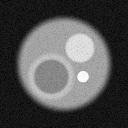
\includegraphics[width=0.2\textwidth]{images/r_3sphere_slice}
	}
	\subfigure[]
	{
		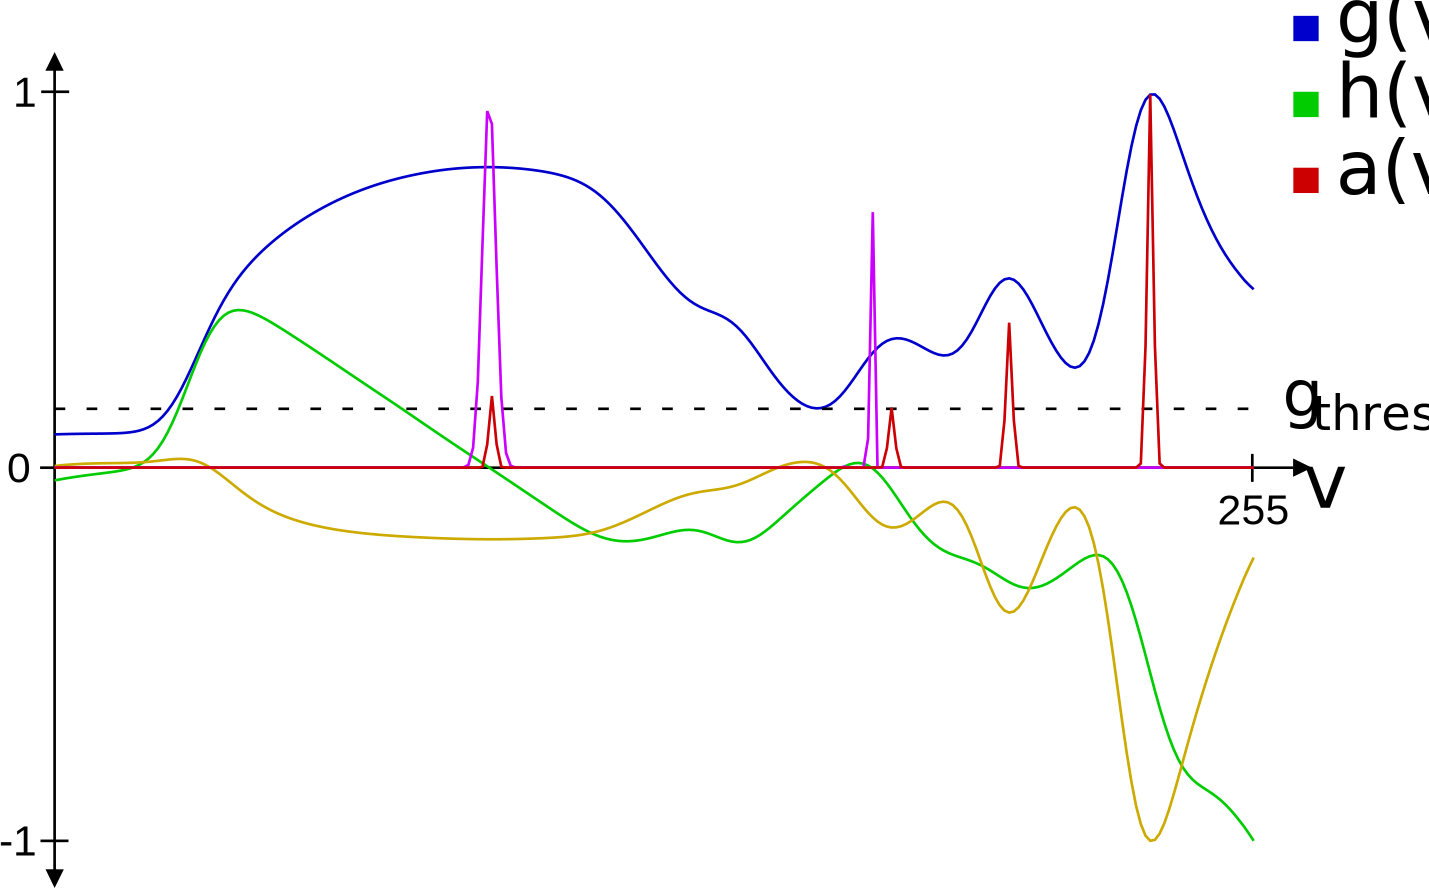
\includegraphics[width=0.75\textwidth]{images/r_3sphere_ft}
	}
	\subfigure[]
	{
		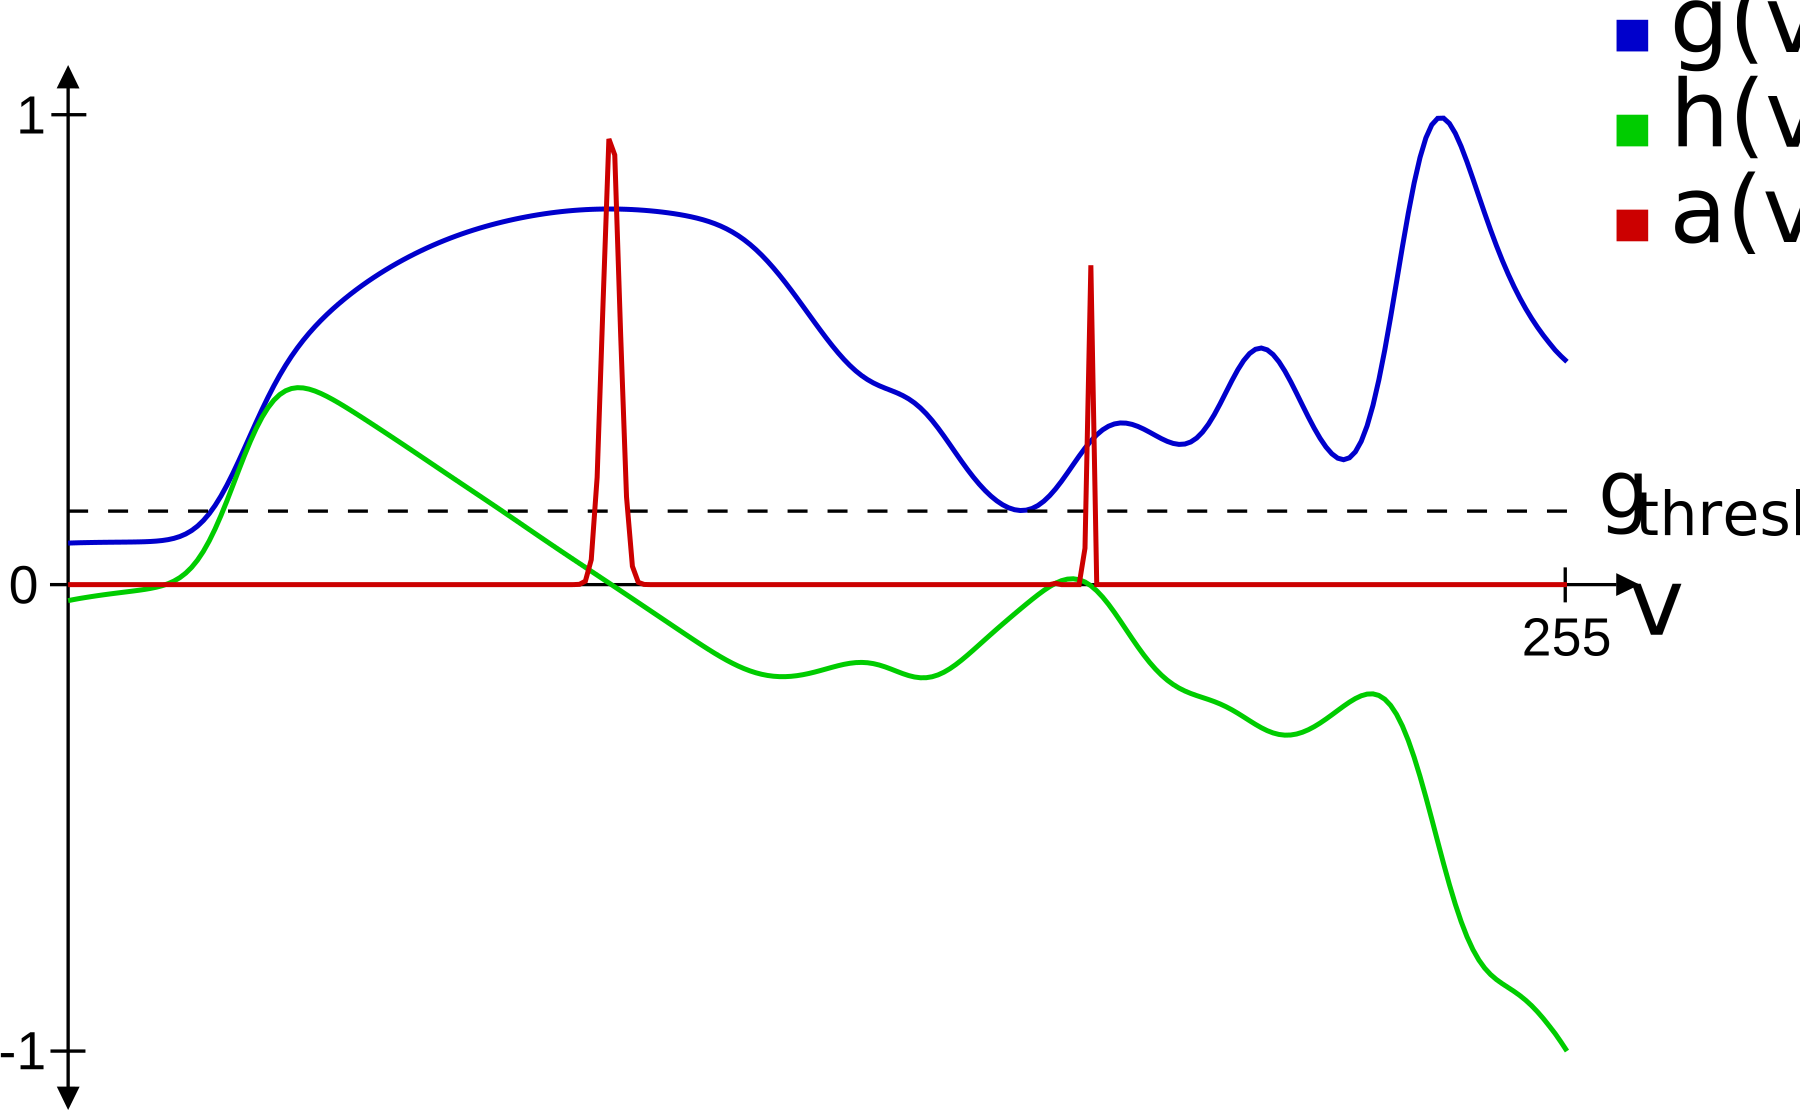
\includegraphics[width=0.45\textwidth]{images/r_g_3sphere}
	}
	\subfigure[]
	{
		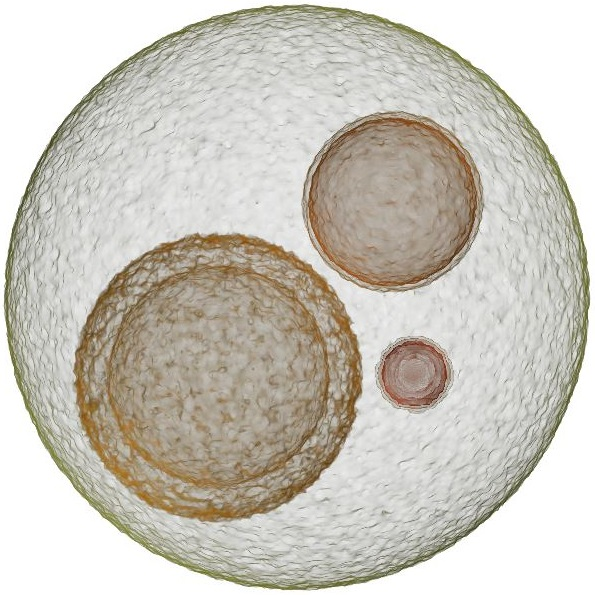
\includegraphics[width=0.45\textwidth]{images/r_m_3sphere}
	}
\end{figure}
	
\section{Malhas Regulares}
\label{sec:result.reg}

\section{Malhas Não Regulares}
\label{sec:result.irreg}